\subsection{Totali}
	\subsubsection{Prospetto orario}
	La distribuzione oraria totale è la seguente:
	
		\begin{table}[!htpb]
			\centering
			\renewcommand{\arraystretch}{2} 
			\rowcolors{2}{gray!25}{white}
			\begin{tabular}{|l c c c c c c|c| }
				\rowcolor{orange!50}
				\hline
				\multicolumn{8}{|c|}{\textbf{Suddivisione delle ore nei vari ruoli}}\\
				\hline
				\textbf{Nominativo} & RES 	& AMM 	& ANA 	& PRO 	& PRG 	& VER 	& \textbf{Totale} \\
				\hline
				\mat 				& 8		& 18	& 10	& 14	& 22	& 27	& 99\\
				\hline
				\pie 				& 12 	& 12	& 13	&16		&27 	&19		&99\\
				\hline
				\mic  				& 8		&12		& 6		&16		&30		& 27	&99\\
				\hline
				\mar  				& 8		&12		& 9		&13		&26 	&31 	&99\\
				\hline
				\daG  				&14		&12		&12 	&14		&14 	&33		&99\\
				\hline
				\daL 				& 8		&15		&11 	&10		&24		&31		&99\\
				\hline
				\gia 				& 8		&18		& 6		&19		&11		&37 	&99\\
				\hline
			\end{tabular}
			\caption{Suddivisione ore totali}
		\end{table}
		~\newline
		Di seguito rappresentata anche in un grafico:
		\begin{figure}[!htpb]
			\centering
			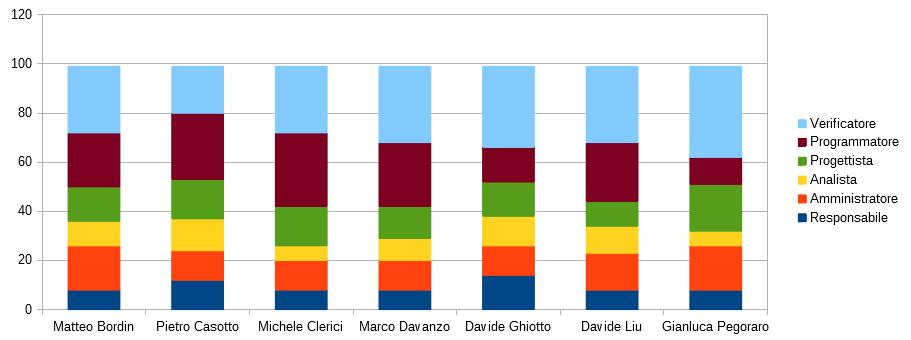
\includegraphics[width=\textwidth]{preventivo/grafico_totali.jpg}
			\caption{Grafico suddivisione oraria}
		\end{figure}
	
	\subsubsection{Conteggio ore}
		La distribuzione delle ore totali nei vari ruoli è la seguente:
		
		\begin{table}[!htpb]
				\centering
			\renewcommand{\arraystretch}{1.8} 
			\rowcolors{2}{gray!25}{white}
			\begin{tabular}{| c c c|}
				\rowcolor{orange!50}
				\hline
				\multicolumn{3}{|c|}{\textbf{Suddivisione delle ore nei vari ruoli}}\\
				\hline
				\textbf{Ruolo} 			& Ore 	& Costo\\
				\hline
				\textbf{Responsabile}	&66 	&1980\\
				\hline
				\textbf{Amministratore}	&99 	&1980\\
				\hline
				\textbf{Analista}		&67 	&1675\\
				\hline
				\textbf{Progettista}	&102 	&2244\\
				\hline
				\textbf{Programmatore}	&154 	&2310\\
				\hline
				\textbf{Verificatore} 	&205 	&3075\\
				\hline
				\textbf{Totale} 		&693	&13264\\
				\hline 
			\end{tabular}
			\caption{Ore e costi totali }
		\end{table}
		~\newline Di seguito rappresentata anche in un grafico:
		\begin{figure}[!htpb]
			\centering
			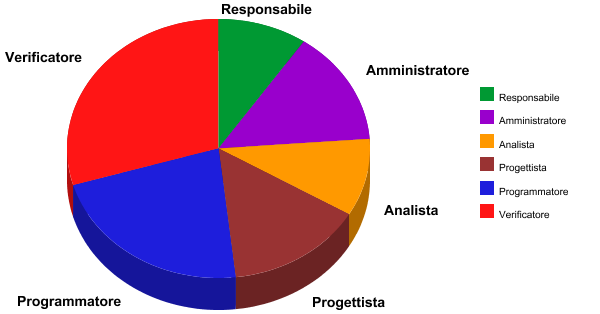
\includegraphics[scale=0.8]{preventivo/torta_totali.png}
			\caption{Grafico suddivisione ruoli}
		\end{figure}
	\clearpage
